\chapter{Wireless protocols}
\label{chap:wireless}

bla bla

In this chapter, I will describe the Industrial, Scientific and Medical (ISM) 2,4 \(GHz\) radio band in \autoref{sec:ism}.
After that, I will demonstrate each wireless protocol starting with Bluetooth Low Energy in \autoref{sec:ble},
Zigbee in \autoref{sec:zig}, and finally Thread/OpenThread in \autoref{sec:ot}.
\autoref{sec:15_4} will provide an overview of the IEEE 802.15.4 radio specification, of which both Zigbee and Thread is based on.

\section{ISM radio band}
\label{sec:ism}

\section{Bluetooth Low Energy}
\label{sec:ble}

Bluetooth is a low-power, short-range wireless technology developed initially for replacing cables when
connecting devices like mobile phones, headsets, and computers.
It has since evolved into a wireless standard for connecting electronic devices to
form Personal Area Networks (PANs) and ad hoc networks. \cite{Dideles03}

Bluetooth is one of the most popular commodity radios for wireless devices.
As a representative of the frequency hopping spread spectrum radios,
it is a natural alternative to broadcast radios in the context of sensor networks. \cite{Leopold03}

The Bluetooth Special Interest Group (SIG) oversees
the Bluetooth standard and has a membership of over 38,000 companies as of 2023. \cite{bt_history}
The initial specification was made available in 1999.
Since then, the SIG released five core specifications, 5.4 being the latest adoption in 2023. \cite{bt_spec_history}

This thesis will focus mainly on Bluetooth Low Energy due to
its similarity in functionality and utilization to Zigbee and Thread/OpenThread.

blab bla.\cite{ble_primer23}.

\subsection{Introcution}
\label{ble:int}
The Bluetooth 4.0 Core Specification introduced Bluetooth Low Energy (BLE).
It is tempting to represent itself as a smaller and highly optimized version of
its bigger brother, classic Bluetooth. In reality, BLE has an entirely different lineage and design goals.
Initially known as Wibree and created by Nokia, the Bluetooth SIG ultimately embraced the technology.
The focus was to develop a radio standard with the lowest possible power consumption,
specifically optimized for low cost, low bandwidth, low power, and low complexity. \cite{Townsend14}

\subsection{Architecture}
\label{ble:ow}

According to Townsend et al., the Bluetooth Low Energy device can be categorized into
three primary blocks: controller, host, and application.
Each block has one or more layers, as shown in \autoref{fig:ble_arch}.

\begin{figure}[!ht]
    \centering
    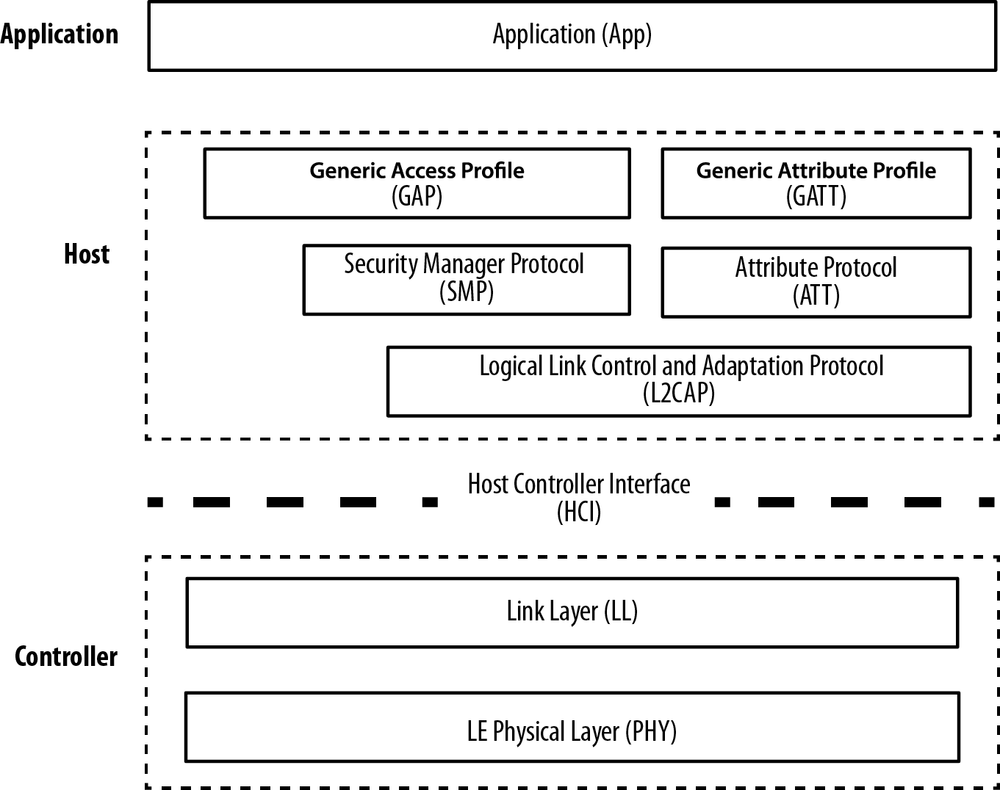
\includegraphics[width=150mm, keepaspectratio]{figures/ble_arch_from_townsend.png}
    \caption{The BLE protocol stack. (Source: Figure 2-1 \cite{Townsend14})}
    \label{fig:ble_arch}
\end{figure}

The layers defined in \autoref{fig:ble_arch} provide the required functionality to operate.

The Controller contains the Physical Layer (PHY) and the Link Layer (LL).
These hold all the responsibility for operating the physical radio channel. 
Also, these layers are specialized by the LE standard keeping the Host
layer more-or-less the same as Bluetooth Classic.


A device address and an address type identify a device.
An address type indicates that an address can be either public or random.
Both are 48 bits long.
A device shall use at least one type of device address but can use
both simultaneously.
Public and random addresses are explained under the Link layer in section 2.4.

In BLE, Generic Access Profile (GAP) defines specific roles for each device.
These roles are: broadcaster, observer, peripheral, and central.
A device may support multiple roles but only one at a given time.
Each role specifies the requirements for the underlying Controller.
\autoref{ble:gap} explains GAP in more detail.


\subsection{Physical layer}
\label{ble:phy}

The physical layer (PHY) contains all necessary analog communication circuitry.
The radio uses the 2.4 GHz ISM band to communicate.
This band is divided into 40 channels or subbands from 2.400 GHz to 2.4835 GHz,
each subband using 2 MHz of bandwidth. (Yin et al., 2019)
This division can be seen in \autoref{fig:ble_phy}.
There are three dedicated advertising subbands for connection setup and
broadcast messages; the remaining 37 are known as general-purpose channels.

\begin{figure}[!ht]
    \centering
    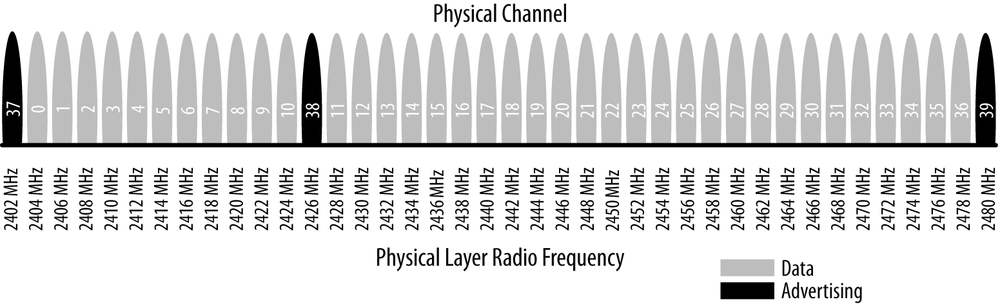
\includegraphics[width=150mm, keepaspectratio]{figures/ble_phy.png}
    \caption{Channel allocation. (Source: Figure 2-2 \cite{Townsend14})}
    \label{fig:ble_phy}
\end{figure}

J. Yin et al. \cite{Yin:19} showed that from Core Specification 5, a novel
modulation scheme was introduced in the standard.
This feature allowed radio modules to use up all 2 MHz of bandwidth,
thus significantly increasing the maximum throughput.

\subsection{Link layer}
\label{ble:link}
Part B of the Core Specification's volume six (Low Energy Controller volume)
defines the Bluetooth Low Energy Link Layer's specification.

The Link Layer is the component that directly communicates with the PHY.
It is typically a blend of custom hardware and software solutions. \cite{Townsend14}

The hardware part usually implements all computationally intensive tasks,
such as CRC generation/validation, random number generation, and AES encryption. 

The software part of this layer is the only hard real-time part of
the whole stack because it has to match the radio hardware's timings
based on the PHY layer's specifications.

The Link Layer can be thought of as a state machine in operation.
In Figure 3, the representation of this state machine can be seen.
The Link Layer may have multiple instances of this state machine but shall have at least one supporting Advertising or Scanning.\cite{bt40}

The Core Specification 5.2 introduced two (2) new states:
Synchronization and Isochronous Broadcasting.

The Air Interface protocol defines the inner working of each state.
This interface consists of multiple access schemes, device discovery,
and Link Layer connection methods.

In the case of multiple state-machine instances, the first version of the
specification (4.0) prohibited certain combinations of states (and roles).
Table 1 specifies the allowed and prohibited state machine combinations.
From the release of Core Specification 5.2, an implementation may support
any combination of states and roles. The only criterion is that any two (2)
devices shall not have more than one connection between them. \cite{bt52}


\subsubsection{Physical channel selection}
\label{ble:link:sel}
After the introduction in Core Specification 5, there are two algorithms for
channel selection.
The initial algorithm (called Channel Selection Algorithm \#1) only supports
channel selection for connection events.
Algorithm \#2 can be used for connection and periodic advertising events.
J. Yin et al. showed that this update significantly enhanced the robustness
of the protocol. (Yin, 2019)

\subsubsection{Link Layer Control protocol}
\label{ble:link:llcp}
The Link Layer Control protocol (LLCP) is used to control and
negotiate aspects of the operation of a connection between two Link Layers.
This includes procedures for control of the connection, starting and pausing
encryption, and other link procedures. \cite{bt40}

One of the most significant procedures is the Channel Map Update Procedure.
This ensures that upon a physical channel update (initiated by
frequency hopping), both the master and the slave stay in sync
with the physical channel index.

% \usepackage{multirow}
\begin{table}[]
    \begin{tabular}{lllllll}
    \multicolumn{2}{l}{\multirow{2}{*}{Multiple State and Role}}  & \multirow{2}{*}{Advertising} & \multirow{2}{*}{Scanning} & \multirow{2}{*}{Initiating} & \multicolumn{2}{l}{Connection} \\
    \multicolumn{2}{l}{}                                          &                              &                           &                             & Master Role    & Slave Role    \\
    \multicolumn{2}{l}{Advertising}                               & Prohibited                   & Allowed                   & Allowed                     & Allowed        & Allowed       \\
    \multicolumn{2}{l}{Scanning}                                  & Allowed                      & Prohibited                & Allowed                     & Allowed        & Allowed       \\
    \multicolumn{2}{l}{Initiating}                                & Allowed                      & Allowed                   & Prohibited                  & Allowed        & Prohibited    \\
    \multicolumn{1}{c}{\multirow{2}{*}{Connection}} & Master Role & Allowed                      & Allowed                   & Allowed                     & Allowed        & Prohibited    \\
    \multicolumn{1}{c}{}                            & Slave Role  & Allowed                      & Allowed                   & Prohibited                  & Prohibited     & Prohibited   
    \end{tabular}
    \caption{Link Layer State Machine limitations (obsolate)}
    \label{tab:llstate_limit}
    \end{table}

\subsection{Host Controller Interface}
The Host Controller Interface (HCI) connects the Controller (low-level)
and Host (high-level) parts of the BLE stack.
It contains a technology-independent logical command interface structure
(HCI driver) and a Host Controller Transport Layer.
The HCI provides a uniform interface for accessing a Bluetooth Controller's
capability.

According to the standard, separating was necessary to keep the HCI driver
independent of the underlying transport technology.
Currently, in the latest standard (Core Specification 5.4), there are four (4)
different technologies defined for the transport layer:
UART, USB, Secure Digital (SD), and Three-wire UART.

\subsection{Logical Link Control and Adaption Protocol}
The Bluetooth logical link control and adaptation protocol (L2CAP)
supports higher-level protocol multiplexing, packet segmentation and
reassembly, and the conveying of quality of service information. 

Packet segmentation is necessary because data must fit into 27-byte maximum
payload size of the BLE packets on the transmit side. (Townsend, 14)
On the reception path, this procedure has to be reversed.

The Bluetooth logical link control and adaptation protocol (L2CAP) supports
higher-level protocol multiplexing, packet segmentation and reassembly,
and the conveying of quality of service information.
The protocol state machine, packet format, and composition are described
in this document. (Townsend, 14)


\subsection{Generic Access Profile}
\label{ble:gap}
The Generic Attribute Profile (GATT) builds on the Attribute Protocol (ATT)
and adds a hierarchy and data abstraction model on top of it.
In a way, it can be considered the backbone of BLE data transfer because
it defines how data is organized and exchanged between applications.



\subsection{Generic Attibute Profile}
\label{ble:gatt}

\section{IEEE 802.15.4}
\label{sec:15_4}

bla bla

\section{Zigbee}
\label{sec:zig}

\subsection{Introduction}
\label{zb:into}
Zigbee is a wireless communication protocol specifically designed for
applications requiring low-power consumption and short-range communication.
It operates on the IEEE 802.15.4 standard and provides a reliable and efficient way
for devices to connect and communicate with each other.
Zigbee is a frequently used technology in home automation, industrial control systems,
and various other applications related to the Internet of Things (IoT).
It supports mesh networking, allowing devices to relay data to extend the network
coverage. Zigbee is known for its low power consumption, simple implementation, and
ability to support a large number of devices in a network.

The Zigbee Alliance created the first version of the specification back in 2004.
In 2022, the alliance renamed itself to Connectivity Standards Alliance.
In 2023, more than 400 companies are actively involved in the alliance. \cite{csa:members}

The first Zigbee specification was released in 2004.
There have been three iterations of the specification, namely Zigbee-2004 (now deprecated), Zigbee-2006, and Zigbee-2007.
In 2023, the latest release is Zigbee-2007 Revision 23.

The Zigbee-2007 specification introduced a new stack called ZigBee Pro. The main difference is in the network layer.
The ZigBee stack is formed around a central coordinator and uses tree addressing to establish a network. Meanwhile,
the Pro version uses stochastic addressing to avoid limitations with a tree. \cite{zigbee:silabs:ug103:2}

The Pro stack implements new features in the routing protocol, such as network-level multicast, many-to-one, and source routing.
Other features are fragmentation, asymmetric link handling, frequency agility, PAN ID conflict resolution, and multiple security levels.
Silicon Labs states that using a Pro network improves stability and reliability.

Both the Pro and the original stack can interoperate but with limitations.
If a Pro coordinator forms a network, the network can only contain Pro routers.
Any stack can act as an end device. \cite{zigbee:silabs:ug103:2}

This thesis will be based on ZigBee Pro Revision 21. This version of the specification is also called ZigBee 3.0.

ZigBee 3.0 contains a new document called Base Device Behavior Specification (BDB).
It possesses mandatory and optional application layer behavior for any ZigBee product. \cite{ti:new:19}, \cite{Morgner:2017}

\subsection{Network}
\label{zb:net:intro}

A Zigbee network is made up of three different types of nodes: Coordinator, Router, and End Device. \cite{Whitehurst:14}

A Zigbee network can be configured to support different topologies: star, tree, and mesh. \autoref{zb:network:topologie} shows the difference between the topologies.

\begin{figure}[!ht]
    \centering
    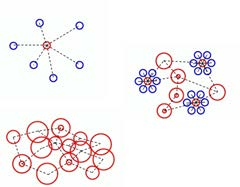
\includegraphics[width=50mm, keepaspectratio]{figures/zigbee-topology-ug103-02-fundamentals-zigbee.jpg}
    \caption{Star, Full Mesh, and Hybrid Mesh topologies. Source(\cite{zigbee:silabs:ug103:2})}
    \label{zb:network:topologie}
\end{figure}

\subsection{Architecture}
\subsection{Network layer}
\subsection{Application layer}

The ZigBee application layer consists of the APS sublayer, the ZDO, and the defined by manufacturer application objects. (Wang et al., 2016)
\cite{nxp:2016}

\subsubsection{Application Support Sub-layer}

The application support sub-layer (APS) provides an interface between the NWK and the application layer through services for ZDO and application objects. 

The APS can be divided into two services: data service and management service. The data service is APS Data Entity (APSDE), and the management service is APS Management Entity (APSME).

The APSDE is responsible for payload conversion, address filtering, reliability, and fragmentation. Once a connection is built up, it is the transport layer between two or more devices.

The other service, the APSME, allows an application to interact with the stack. It is responsible for AIB, binding, security, and group management.


\subsubsection{Application Framework}

The application Framework provides a hosting environment for application objects on a Zigbee device.
A developer can define up to 240 distinct application objects, each identified by an endpoint address from 1 to 240. 

Index 0 is reserved for communication with ZDO, and index 255 is considered the broadcast address.
For future use, the alliance reserved the index range from 241 to 254.

\subsubsection{Zigbee Device Object}
Zigbee device object interfaces the application objects, the device profile, and the APS.
For the application objects, it provides device control and network functions.
Other functions are address management of the device, discovery, binding, and security. (Wang et al., 2016)

The ZDO is responsible for initializing the APS sublayer, the NWK layer, and the Security Service Provider. Also, the ZDO defines the role of the device within a ZigBee network.

\subsection{Cluster Library}

%\url{https://www.academia.edu/73196763/A_Survey_of_ZigBee_Wireless_Sensor_Network_Technology_Topology_Applications_and_Challenges}
%\url{https://issuu.com/ijtsrd.com/docs/399_literature_survey_on_zigbee_iee}
%\url{https://www.sciencedirect.com/topics/engineering/zigbee-protocol}

\section{Thread/OpenThread}
\label{sec:ot}

\subsection{Introduction}
\label{sec:ot:intro}
Thread is intended to be an open standard, and the protocol is built by incorporating many
current and proposed standards.\cite{unwala:2018}
Anyone can download the complete specification from the Thread Group website. \cite{thread:130}

As mentioned, the Thread Group develops and maintains the protocol.
Thread Group is a not-for-profit organization formed by seven companies:
ARM (Softbank), Big Ass Fans, Freescale (NXP), Nest Labs (Google), Samsung, Silicon Labs, and Yale Locks.
More than 200 companies, such as Apple, Google, and Amazon, are forming the Thread Group. \cite{thread:members}

This thesis uses the Thread specification, v1.3.0 2023.

\subsection{Private Area Network}
\label{sec:ot:pan}
In a Thread network, there are two types of devices (nodes): Full Thread Device (FTD) and Minimal Thread Device (MTD). FTDs can communicate with each other and with their attached MTD children. MTDs can only communicate with the parent FTD.

A Thread Device can act in six different roles.
\begin{enumerate}
    \item Active Router
    \item Router.Eligible End Device (REED)
    \item Full End Device (FED)
    \item Minimal End Device (MED)
    \item Sleepy End Device (SED)
    \item Synchronized Sleepy End Device (SEED)
\end{enumerate}

In order to create a network, the initial node must select an IEEE 802.15.4 channel and
a PAN Identifier (PAN ID).
The forming node becomes the PAN's first Router and selects a Rouder ID for itself.

The topology is based on the number of Routers in the Thread Network.
If there is only one Router, then a basic star topology with a single Router is formed.
A mesh topology is automatically formed if there is more than one Router.
\autoref{fig:ot:network} shows a basic topology.

\begin{figure}[!ht]
    \centering
    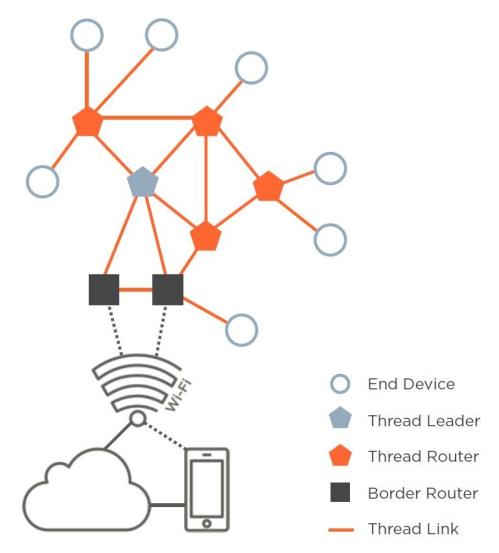
\includegraphics[width=100mm, keepaspectratio]{figures/thread-topology-ThreadNetworkFundamentals_633_4.jpg}
    \caption{Channel allocation. (Source: Figure 3 \cite{thread:nfwp})}
    \label{fig:ot:network}
\end{figure}

The Mesh Commissioning Protocol (MshCoP) manages how a new device can join a Thread Network.
A commissioner device is an elected authentication server.
This device can be a cell phone, a cloud service, or an FTD.
There can only be one commissioner node in a PAN, and the Thread Management Protocol manages it.

A new device that wants to join the network is called Joiner.
A Joiner Router is a node that can act as a Router and is one hop away from the Joiner.

There are two main approaches to commissioning:
\emph{external} if the commissioner is connected to the Thread Network via a Border Router or
\emph{native} if the commissioner is in the Thread Network. 
Different approaches are shown in \autoref{fig:ot:commissioning}.

\begin{figure}[!ht]
	\centering
	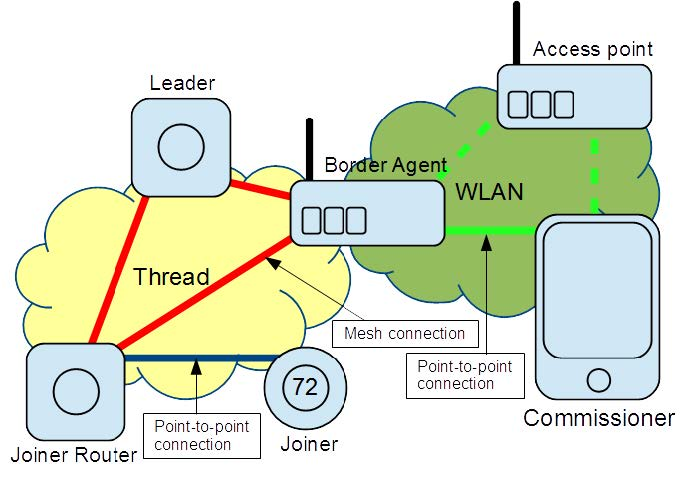
\includegraphics[width=67mm, keepaspectratio]{figures/external1-Final_12639Thread_1.3.jpg}\hspace{1cm}
	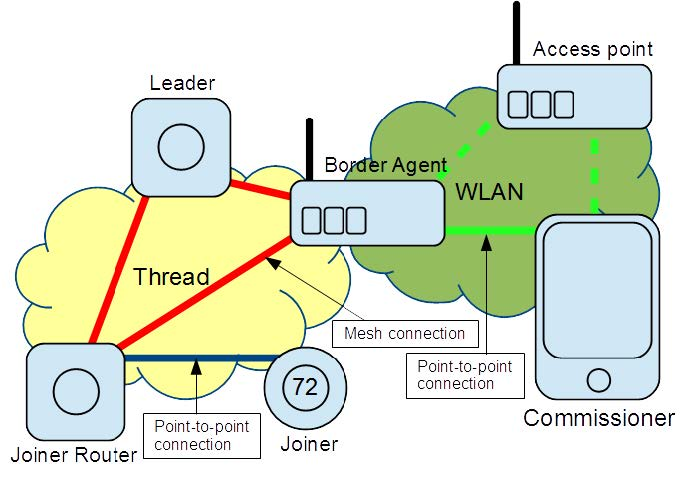
\includegraphics[width=67mm, keepaspectratio]{figures/external1-Final_12639Thread_1.3.jpg}\\\vspace{5mm}
	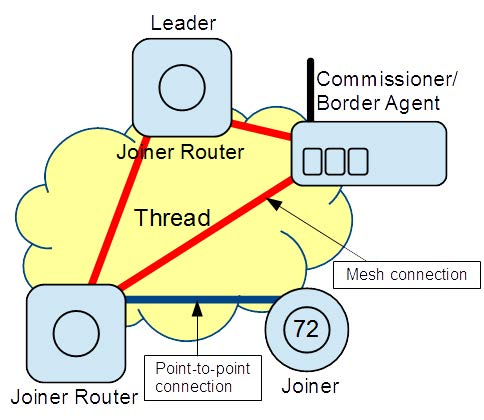
\includegraphics[width=67mm, keepaspectratio]{figures/native1-Final_12639Thread_1.3.jpg}\hspace{1cm}
	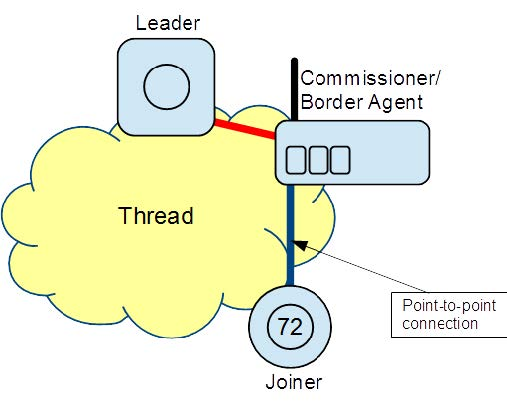
\includegraphics[width=67mm, keepaspectratio]{figures/native2-Final_12639Thread_1.3.jpg}
	\caption{External and Nativ commissioning. (Source: \cite{thread:130})}
	\label{fig:ot:commissioning}
\end{figure}


State machines can define the behavior of the Joiner (see \autoref{fig:ot:joiner-sm}),
the Joiner Router (see \autoref{fig:ot:joiner-rt-sm}), and the Commissioner (see \autoref{fig:ot:commissioner-sm}).

\begin{figure}[!ht]
    \centering
    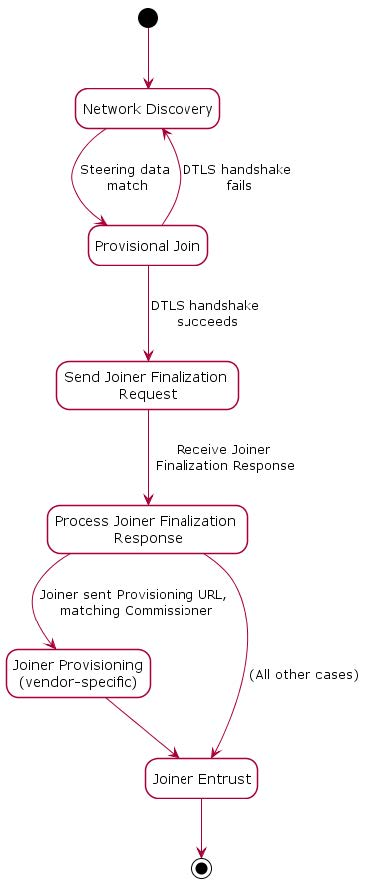
\includegraphics[height=150mm, keepaspectratio]{figures/joiner-sm-Final_12639Thread_1.3.jpg}
    \caption{The Joiner's state machine (Source: \cite{thread:130})}
    \label{fig:ot:joiner-sm}
\end{figure}

\begin{figure}[!ht]
    \centering
    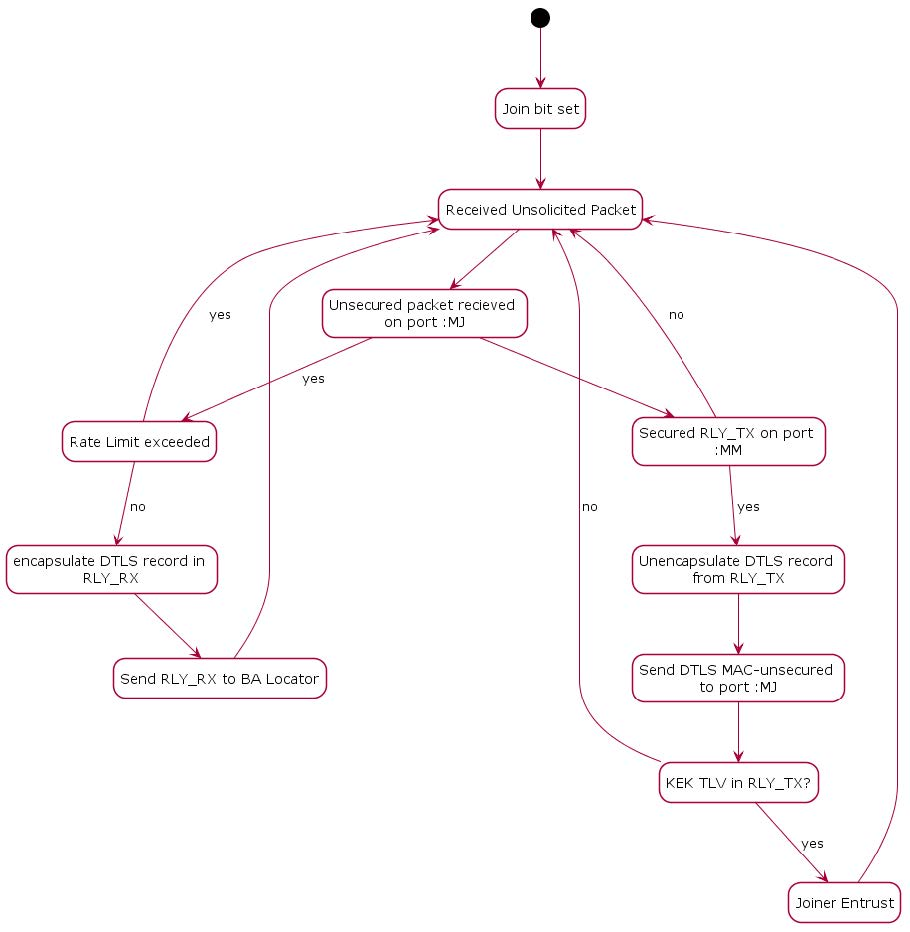
\includegraphics[width=100mm, keepaspectratio]{figures/joiner-rt-smFinal_12639Thread_1.3.jpg}
    \caption{The Joiner Router's state machine (Source: \cite{thread:130})}
    \label{fig:ot:joiner-rt-sm}
\end{figure}

\begin{figure}[!ht]
    \centering
    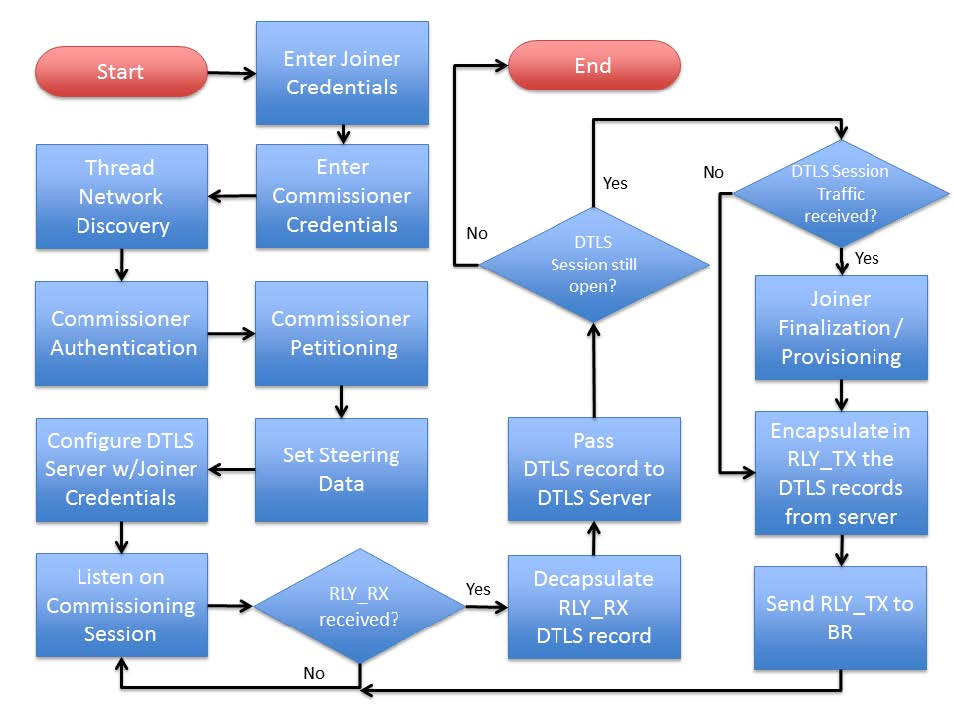
\includegraphics[width=100mm, keepaspectratio]{figures/commissioner-sm-Final_12639Thread_1.3.jpg}
    \caption{The Commissioner's state machine (Source: \cite{thread:130})}
    \label{fig:ot:commissioner-sm}
\end{figure}

%\url{https://ieeexplore.ieee.org/abstract/document/8767079}
%\url{https://ieeexplore.ieee.org/abstract/document/8373620}
%\url{https://ieeexplore.ieee.org/abstract/document/10022228}
%\url{https://ieeexplore.ieee.org/abstract/document/9058170}
%\url{https://dl.acm.org/doi/abs/10.1145/3507657.3528544}
%\url{https://www.diva-portal.org/smash/record.jsf?pid=diva2%3A1040491&dswid=1593}
%\url{https://upcommons.upc.edu/handle/2117/101928}
%\url{https://ieeexplore.ieee.org/abstract/document/8106811}
%\url{https://ieeexplore.ieee.org/abstract/document/8592759}
%\url{https://ieeexplore.ieee.org/abstract/document/8374875}
%\url{https://www.diva-portal.org/smash/record.jsf?pid=diva2%3A1282697&dswid=-3708}
%\url{https://ieeexplore.ieee.org/abstract/document/8586865}
%\url{https://link.springer.com/chapter/10.1007/978-3-030-70080-5_9#Sec8}